\documentclass[a4paper,8pt]{beamer}

\usepackage[utf8]{inputenc}
\usepackage{fontspec}
\usepackage{amsmath}
\usepackage{amssymb}
\usepackage{subfloat}

\usefonttheme{professionalfonts}

\usefonttheme[]{structurebold}

\usetheme{Copenhagen}
\usecolortheme{rose}
\usecolortheme{dolphin}
\useinnertheme{circles}
\useoutertheme{tree}

\setmainfont[Path=/usr/share/fonts/truetype/calibri/,
BoldItalicFont=calibriz.ttf,
BoldFont      =calibrib.ttf,
ItalicFont    =calibrii.ttf]{calibri.ttf}

\newcommand{\BS}[1]{\boldsymbol{#1}}


\title{Generalized Langevin Equation}
\subtitle{Stochastic Differential Equations}
\author{Sankarasubramanian Ragunathan \newline \newline 389851}
\institute{\textbf{RWTH Aachen}}
\date{}


\begin{document}
	\begin{frame}
		\titlepage
		\centering
		
\includegraphics[width=0.2\textwidth]{RWTH_Aachen_University_Logo.eps}
	\end{frame}

	\begin{frame}
		\tableofcontents
	\end{frame}

	\begin{frame}
		\section{Scope of the Project}
		\frametitle{Scope of the Project}
		
		\begin{itemize}
			\item[What?]{Generalized Langevin Dynamics is a modeling technique that can be used to model anomalous diffusive phenomena observed in viscoelastic fluid flow and in biological systems.}
			
			\item[Why?]{Complex physical systems' behavior cannot be captured successfully using the delta-correlated forces used in Langevin Dynamics necessitating the use of GLD.}
			
			\item[Where?]{Applications of GLD include but are not restricted to micro-rheology, biological systems, nuclear quantum effects and systems in which anomalous diffusion arise.}
			
			\item[How?]{The theory behind extended variable GLD is studied and several numerical schemes are also tested to find out the optimal scheme w.r.t. convergence of the solution. \textcolor{red}{If possible, the sensitivity of the solution to the change in the parameters of the extended variable Prony series is also studied.}}
		\end{itemize}
	\end{frame}
	
	\begin{frame}
		\section{Introduction}
		\frametitle{Introduction}
		
		\quad \textbf{Langevin Dynamics} is a modeling technique in which the motion of a set of massive bodies in the presence of a bath of smaller solvent particles is directly integrated, while the dynamics of the solvent are "averaged out".
		
		\quad This approximation leads to drastic reduction in computational cost as the dynamics of the solvent particles no longer need to be fully resolved. With Langevin dynamics, the effect of the solvent is reduced to an instantaneous drag force and a random delta-correlated force felt by the massive bodies.
		
		\quad The drawback with the conventional Langevin dynamics is that the underlying assumptions made to develop the scheme cannot be applied for all scenarios necessitating a more general treatment leading to the usage of \textbf{Generalized Langevin Dynamics}. 
	\end{frame}
	
	\begin{frame}
		\section{Mathematical Fomulation}
		\frametitle{Mathematical Formulation}
		The Ornstein-Uhlenbeck SDE models the momentum of particles undergoing collisions.
		\begin{gather}
			dX = -\gamma X dt + \sigma dW \\
			X = p
		\end{gather}
		The Ornstein-Uhlenbeck SDE equation samples, in the long term, the Gibbs-Boltzmann distribution associated to a single particle in a thermal bath at temperature $T$.
		For a system with $N_{c}$ configurational variables we may write,
		\begin{gather}
			dp_{i} = -\gamma p_{i} dt + \sqrt{2 \gamma k_{B} T m_{i}} dW_{i} 
		\end{gather}
		where $W_{i}$ represents $N_{c}$ individual Wiener processes.
		
		If the Ornstein-Uhlenbeck SDE models the momentum of particles undergoing collisions, it can be complemented by a corresponding differential equation for the position of the form
		\begin{gather}
			dq = m^{-1} p dt
		\end{gather}
		to provide a full description of the motion. This is the key idea in Langevin's model for Brownian motion.
	\end{frame}

	\begin{frame}
		\section{Models for Heat Baths and Langevin's Model for Brownian Motion}
		\frametitle{Models for Heat Baths and Langevin's Model for Brownian Motion}
		Let us derive the Langevin dynamics model for the special case of a heavy particle ($M = 1$) interacting with a large collection of light particles. We assume that we are given a system of $k$ coupled oscillators (a "heat bath") in contact with a distinguished particle (Here, the special "heavy particle"). The Hamiltonian is given by:
		\begin{gather}
			H = \frac{P^2}{2M} + \sum_{i=1}^{k} \frac{p_{i}^2}{2 \mu_{i}} + U(Q) + \frac{1}{2k} \sum_{i=1}^{k} (q_{i} - Q)^2
		\end{gather}
		where $Q$ and $P$ represent the position and momentum of the distinguished particle and $\{q_{i},p_{i}\}$ are the positions and momenta of the particles of the bath, $\mu_{i}$ giving the mass of the $i$th particle.
		The equations of motion for the combined system are:
		\begin{gather}
			\dot{Q} = \frac{P}{M} = P, \quad \quad
			\dot{P} = -U^{'}(Q) - k^{-1} \sum_{i=1}^{k} (Q-q_{i})
			\label{eq:BigQP}
		\end{gather}
		where for $i = 1,2,\dots,k$
		\begin{gather}
			\dot{q_{i}} = \frac{p_{i}}{\mu_{i}}, \quad \quad
			\dot{p_{i}} = \frac{Q-q_{i}}{k}
			\label{eq:SmallQP}
		\end{gather}
	\end{frame}

	\begin{frame}
		Because the above system is linear, we can solve it analytically for $\{q_{i},p_{i}\}$ yielding:
		\begin{gather}
			q_{i}(t) = cos(\Omega_{i}t)q_{i}(0) + \Omega_{i}^{-1} sin(\Omega_{i}t)\frac{p_{i}(0)}{\mu_{i}} +  k^{-1}\mu_{i}^{-1} \int_{0}^{t} {\Omega_{i}^{-1} sin(\Omega_{i}(t-s))Q(s)ds}
		\end{gather}
		where $\Omega_{i} = (k \mu_{i})^{-\frac{1}{2}}$ is the frequency of the $i^{th}$ oscillator. Integrating by parts, we have
		\begin{align}
			\int_{0}^{t} \Omega_{i} sin(\Omega_{i}(t-s))Q(s)ds =& [cos(\Omega_{i}(t-s))Q(s)]_{0}^{t}
			- \int_{0}^{t} cos(\Omega_{i} (t-s))P(s)ds \\
			=& Q(t) - cos(\Omega_{i} t)Q(0) - \int_{0}^{t} cos(\Omega_{i}(t-s))P(s)ds
		\end{align}
		which leads to
		\begin{gather}
			\notag q_{i}(t) - Q(t) = cos(\Omega_{i}t)q_{i}(0) + \Omega_{i}^{-1} sin(\Omega_{i}t)\frac{p_{i}}{\mu_{i}} \\ - cos(\Omega_{i}t)Q(0) - \int_{0}^{t} cos(\Omega_{i}(t-s))P(s)ds
		\end{gather}
	\end{frame}

	\begin{frame}
		Inserting the above equation in Equation \eqref{eq:BigQP}, we get the reduced system given below
		\begin{gather}
			\dot{Q} = P \\
			\dot{P} = -U^{'}(Q) - k^{-1} \sum_{i=1}^{k} (Q-q_{i}) = -U^{'}(Q) + f(t) - \int_{0}^{t} \psi (t-s)P(s)ds
			\label{eq:delaydiff}
		\end{gather}
		where $f(t)$ and $\psi(t)$ are defined as
		\begin{gather}
			f(t) = -k^{-1} \sum_{i=1}^{k} [ cos(\Omega_{i}t)q_{i}(0) + \Omega_{i}^{-1} sin(\Omega_{i}t)\frac{p_{i}(0)}{\mu_{i}} - cos(\Omega_{i}t)Q(0)] \\
			\psi(t) = k^{-1} \sum_{i=1}^{k} cos(\Omega_{i}t)
		\end{gather}
		Here $\psi(t)$ represents the \textbf{\texttt{Memory Kernel}} function. Different choices of sequences of $\Omega_{i}^{(k)}$ will lead to different appearances of the memory kernel function $\psi(t)$
		\begin{block}{Note}
			For large $k$ and for many choices of the frequencies $\Omega_{i}$ and the initial conditions $\{ q_{i}(0),p_{i}(0) \}$, function $f(t)$ will take on the character of a Wiener process; in fact the convergence can be shown in a weak sense.
		\end{block}
	\end{frame}

	\begin{frame}
		\begin{figure}[H]
			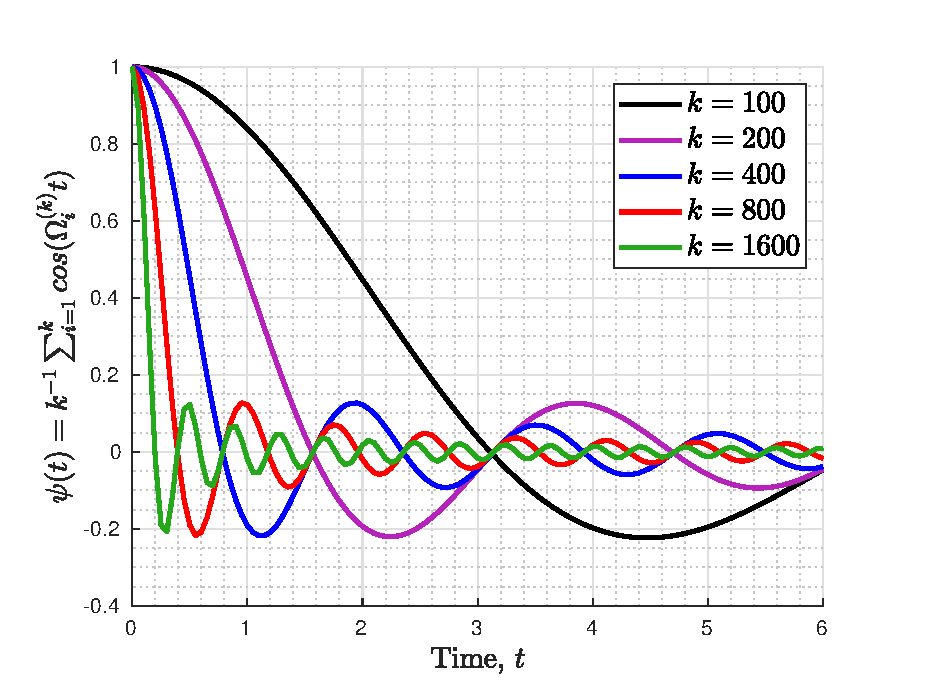
\includegraphics[width=0.75\textwidth]{../Code/GeneralPlots/MemoryKernel.eps}
			\label{fig:memorykernel}
			\caption{Memory Kernel function $\psi(t)$ plotted for different frequencies $k$}
		\end{figure}
	\end{frame}

	\begin{frame}
		If sufficiently high frequency components are present, then the mass of the memory kernel is typically found to be localized around 0; in such a situation of rapid decay it is found that one may replace the function $\psi(t)$ by a Dirac-Delta function scaled by a positive coefficient $\gamma$; we say that the system is Markovian or memory-less in this situation and we replace the delay-differential equation \eqref{eq:delaydiff} by the SDEs
		\begin{gather}
			dQ = Pdt \\
			dP = -U^{'}(Q)dt + \sigma dW - \gamma P dt
		\end{gather}
		where we have viewed the function $f(t)$ as being approximated by a Wiener increment. This system then leads to an approximate model referred to as \emph{Langevin Dynamics}. In our case, we will consider the \emph{Generalized Langevin Dynamics} where we don't approximate the delay-differential equation.
	\end{frame}

	\begin{frame}
		\section{Generalized Langevin Equation}
		\frametitle{Generalized Langevin Equation}
		We already saw the case where the GLE equation was obtained as an intermediate step in deriving the Langevin dynamics. In some cases, we might want to model the properties of the heat bath and the resulting memory kernel thus necessitating us to use GLE for simulations.
		
		The equations of GLE are normally written in the form
		\begin{gather}
			d\BS{q} = \BS{M}^{-1} \BS{p} dt \\
			d\BS{p} = -\nabla U(\BS{q}) dt - \int_{0}^{t} \BS{\Gamma}(t-s) \BS{p}(s) ds dt + d\BS{B}
		\end{gather}
		subject to initial conditions $\BS{q}(0) = \BS{q}_{0}$,$\BS{p}(0) = \BS{p}_{0}$. Here $\BS{\Gamma}(t) = (\gamma_{ij}(t))$ is a $N_c \times N_c$ matrix-valued function of $t$ which we refer to as the \textbf{\texttt{memory kernel}}. The term
		\begin{gather}
			\BS{F}_d = - \int_{0}^{t} \BS{\Gamma}(t-s) \BS{p}(s) ds dt
		\end{gather}
		represents a drag force acting on the system due to the interaction with the particles of the bath. $d\BS{B}$ is the increment of the colored-noise (non-Gaussian) stochastic process. Often this increment is treated formally as an impulse $\BS{R}(t)dt$, where $\BS{R}$ is referred to as a \textbf{\texttt{Random Force}} which is related to a Stochastic process.
	\end{frame}
\end{document}